\documentclass[12pt]{article}
\usepackage[utf8]{inputenc}
\usepackage{float}
\usepackage{amsmath}
\usepackage[hmargin=3cm,vmargin=6.0cm]{geometry}
%\topmargin=0cm
\topmargin=-2cm
\addtolength{\textheight}{6.5cm}
\addtolength{\textwidth}{2.0cm}
%\setlength{\leftmargin}{-5cm}
\setlength{\oddsidemargin}{0.0cm}
\setlength{\evensidemargin}{0.0cm}
\usepackage{graphicx}
\graphicspath{ {images/} }


\centering
\begin{document}

\section*{CENG435 HW2 REPORT} 

Full Name :  \ Şevki Kocadağ\
Student ID :  \ 1869049 \
\\
Full Name :  \ Barış Yerci \
Student ID :  \ 2099513 \


\begin{quote}
$\ \  \ \ \ \ \ $In this homework, we have implemented the RDT over UDP and SCTP.
These rectangle means a Node in the network.
Node s is implemented as a Source which use UDP sockets for RDT.
Node r1 is implemented as a router with route command.
Node r2 is also implemented as a router with route command.
Node d is implemented as a Destination which use UDP socket for sending ACK message.
\end{quote}


\
\centering
\large
\textbf{Followed Topology}

\
\
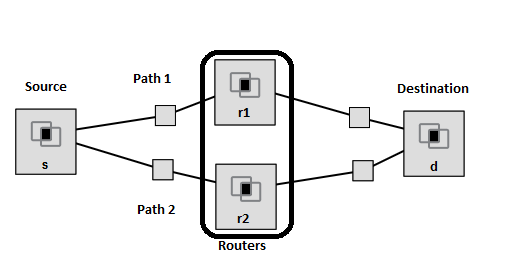
\includegraphics[width = 170mm, height = 40mm]{topology}

\
\


\normalsize
\begin{quote}
$\ \  \ \ \ \ \ $For the first experiment, our RDT send all file on path 2. r2 just route all packets to d. We arrange this routing with "route add -host 10.10.4.2 gw 10.10.4.1" and "route add -host 10.10.3.1 gw 10.10.3.2" on r2. For the other experiment, our RDT send file on half on r1 and half on r2. We arrange r2 same as experiment one and r1 with "route add -host 10.10.2.2 gw 10.10.2.1" and "route add -host 10.10.1.1 gw 10.10.1.2" on r2.
\\
Also, We prepared shell scripts which are named as "r1.sh" for Router 1 and "r2.sh" for Router 2 to run easily.
\end{quote}

\section*{Design and Implementation}
\begin{quote}
$\ \  \ \ \ \ \ $ Firstly, we take as input what experiment will be solved and create  thread as much as we need.Then read all file which we send and if the second experiment will be solved, we divide file into two equal size and send them first and second thread. We implement Go-back-N struct with window size is five. Go-back-N can be explained as a specific instance of the automatic repeat request (ARQ) protocol, in which the sending process continues to send a number of frames specified by a window size even without receiving an acknowledgement (ACK) packet from the receiver.It is a special case of the general sliding window protocol with the transmit window size of N and receive window size of 1. It can transmit N frames to the peer before requiring an ACK. We send 1000 byte in every packet. First 100 byte of this packets is header. Header contains client address, destination address, packet number, checkSum, closure flag. Our RDT work like that first of all, source send five packet and if destination receive packet, it calculate checksum and compare header checksum.If these two checksums  are not equal ,this mean packet is corrupted so destination does not send ack message to source. If the head of window in Go-back-N struct get timeout, source send all file in window. When the last packet send closure flag set to one and sockets close in source and destination.

As for Stream Control Transmission Protocol (SCTP), according to  Tuexen et al., SCTP defined that "SCTP provides some of the same service features of both UDP and TCP: it is message-oriented like UDP and ensures reliable, in-sequence transport of messages with congestion control like TCP; it differs from these in providing multi-homing and redundant paths to increase resilience and reliability."(May 2013)\\
Since there are multi-homing and no multi-homing experiments, we used thread in SCTP for multi-homing. Therefore, we can divide data and give them to threads to sent to destionation. Also, one client and server programming file (python) are enough for multi-homing or non-multi-homing experiments. Just before running, we can determine it is multi-homing or not. For example, \\
\begin{center}
$ server\_sctp.py\ experimentNo$
\end{center}
To implement SCTP in Python, we need to install PySctp library in GitHub. Also, we prepared a shell script to setup easily.
  

  
\end{quote}


\section*{Graph and Comment}
\
\
\begin{quote}
$\ \  \ \ \ \ \ $ As we can see from below graphs, our RDT is faster than SCTP .There are several reason for that. First of all, our time out may be shorter than SCPT class, so SCTP waits more time. Other reason might be header.Our header 100 byte, but we do not know how many byte SCTP class header is. Final reason may be that memory using when server write sending file to output file.
\end{quote}

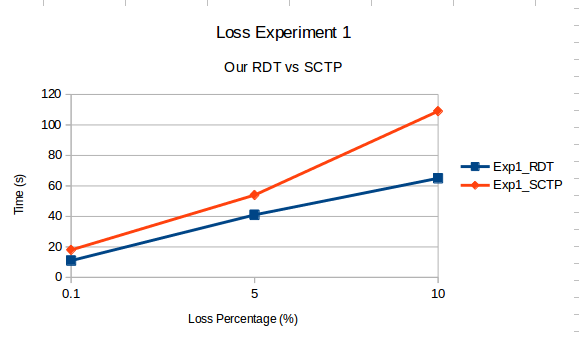
\includegraphics[width = 180mm, height = 120mm]{LossExperiment1}


\begin{quote}
$\ \  \ \ \ \ \ $ All reason from above are valid for multi-hommed (experiment 2 graphs), but there are more reason. Our threads for sending input file may be better implemented than SCTP class which we use. We may say that our RDT is more efficient than SCTP
\end{quote}

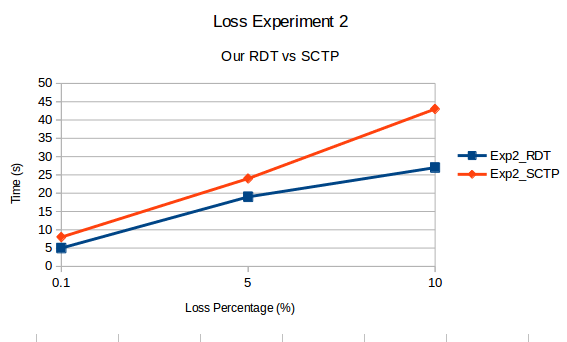
\includegraphics[width = 180mm, height = 120mm]{LossExperiment2}

\begin{quote}
$\ \  \ \ \ \ \ $ As we can see from below graph, our RDT is faster than SCTP .There are several reason for that. First of all, our RDT may be faster calculated checksum than SCTP class. We use checksum from special class from python class. Checksum just know destination and source in our RDT, but SCTP class handle checksum from inside.This corruption checking systems cause delay.



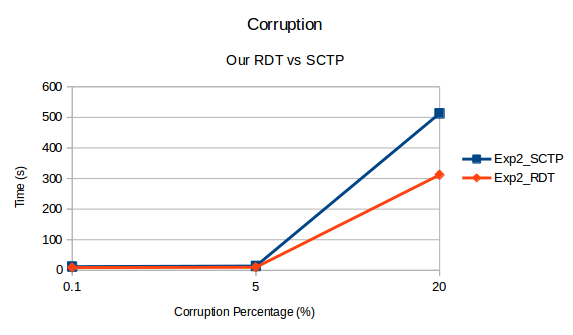
\includegraphics[width = 180mm, height = 90mm]{Corruption}
\end{quote}

\begin{quote}
$\ \  \ \ \ \ \ $ As we can see from below graph, our RDT is slower than SCTP because we use Go-back-N, so when packets get timeout ,we send all window again and SCTP do not. In addition, SCTP may be optimize window.  



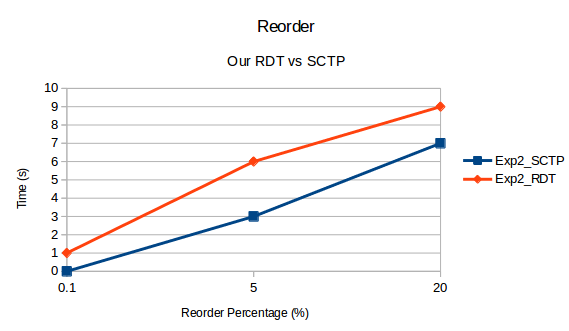
\includegraphics[width = 180mm, height = 100mm]{Reorder}
\end{quote}

\begin{quote}
\newpage
$\ \  \ \ \ \ \ $In conclusion, all these graphs show us when corruption or loss occur,our RDT tolerate faster than SCTP, but when reorder occur, because of the Go-back-N struct we could not tolerate as fast as  SCTP.
\end{quote}
\section*{Reference}

\begin{quote}
Tuexen, Michael; Randall R. Stewart (May 2013). UDP Encapsulation of Stream Control Transmission Protocol (SCTP) Packets for End-Host to End-Host Communication. IETF. RFC 6951. https://tools.ietf.org/html/rfc6951.
\end{quote}
\end{document}
\grid
\grid
